\documentclass{beamer}
\usepackage{ctex, hyperref}
\usepackage[T1]{fontenc}
\usepackage{graphicx}
\usepackage{booktabs}
\usepackage{tikz}
\usetikzlibrary{positioning, arrows.meta, shapes.geometric, calc}

% ---- 可修改的元信息（占位）----
\newcommand{\ProjectAuthor}{王新凯 \quad 包家和}
\newcommand{\ProjectInstitute}{}
\newcommand{\ProjectAdvisor}{陈叶芳}

\author{\ProjectAuthor}
\institute{\ProjectInstitute}
\title{面向监控场景的火情识别系统}
\subtitle{基于目标检测与视觉语义模型的多模型融合方案}
% \date{\today}

\usepackage{Westlake}

% 取消 Westlake 主题在每个 section 自动插入目录页，保持 PPT 简洁
\AtBeginSection[]{}
\AtBeginSubsection[]{}

% 配色：沿用主题主色 westlake(#004990)
\definecolor{westlakedark}{RGB}{0,35,75}
\definecolor{westlakelight}{RGB}{232,240,248}

\begin{document}

% ================= 封面 =================
\begin{frame}[plain]
  \titlepage
  \vspace{-0.6em}
  \begin{center}
    \footnotesize 指导教师：\ProjectAdvisor
  \end{center}
\end{frame}

% ================= 第2页 项目背景 =================
\section{项目概述}
\begin{frame}{项目背景}
  \begin{itemize}
    \item 城市消防、工业厂区、林区、地下空间等场景依赖监控摄像头进行火情防范
    \item 人工巡检受实时性与覆盖范围限制，难以持续关注海量监控画面
    \item 火焰与烟雾在尺度、形态、光照和背景上变化明显，单一简单规则难以可靠判断
    \item 目标：利用视觉模型对监控图像进行自动化的火情判断
  \end{itemize}
  \begin{block}{}
    \small 以一张监控图像为输入，自动给出「有火 / 无火」的图像级判断结果。
  \end{block}
\end{frame}

% ================= 第3页 项目目标与主要功能 =================
\begin{frame}{项目目标与主要功能}
  \begin{columns}[t]
    \column{0.33\textwidth}
      \begin{block}{输入}
        \small
        \begin{itemize}
          \item 读取单张或批量监控图像
          \item 支持常见图片格式
        \end{itemize}
      \end{block}
    \column{0.33\textwidth}
      \begin{block}{处理}
        \small
        \begin{itemize}
          \item 检测候选火焰/烟雾区域
          \item 视觉语义模型进一步判断
          \item 多模型信息融合
        \end{itemize}
      \end{block}
    \column{0.33\textwidth}
      \begin{block}{输出}
        \small
        \begin{itemize}
          \item 图像级 0/1 火情结果
          \item 结构化 JSON 文件
          \item 提交前自动校验
        \end{itemize}
      \end{block}
  \end{columns}
  \vspace{0.5em}
  \begin{center}
    \small 输入图像 $\longrightarrow$ 多模型协同推理 $\longrightarrow$ 图像级判断结果
  \end{center}
\end{frame}

% ================= 第4页 系统总体架构 =================
\begin{frame}{系统总体架构}
  \begin{center}
  \begin{tikzpicture}[
    node distance=0.38cm,
    box/.style={rectangle, rounded corners, draw=westlake, fill=westlakelight,
                text width=2.9cm, align=center, minimum height=0.55cm, font=\small,
                inner sep=0.15em},
    wide/.style={text width=4.4cm},
    arr/.style={-{Stealth[length=2mm]}, thick, westlake}
  ]
    \node[box, wide] (img) {监控图像输入};
    \node[box, wide, below=of img] (pre) {图像预处理};

    \node[box, below=0.4cm of pre, xshift=-1.75cm] (det) {目标检测\\（YOLO 系列）};
    \node[box, below=0.4cm of pre, xshift=+1.75cm] (vis) {视觉语义分类\\（SigLIP / DINO）};
    \node[box, below=of det] (crop) {候选区域裁剪};
    \node[box, below=of vis] (local) {局部复核};

    \node[box, wide, below=0.75cm of crop] (fus) {多模型决策融合};
    \node[box, wide, below=of fus] (out) {图像级火情判断（0/1）};
    \node[box, wide, below=of out] (json) {JSON 生成与独立校验};

    \draw[arr] (img) -- (pre);
    \draw[arr] (pre.south) -- (det.north);
    \draw[arr] (pre.south) -- (vis.north);
    \draw[arr] (det) -- (crop);
    \draw[arr] (vis) -- (local);
    \draw[arr] (crop.south) -- (fus.north);
    \draw[arr] (local.south) -- (fus.north);
    \draw[arr] (fus) -- (out);
    \draw[arr] (out) -- (json);
  \end{tikzpicture}
  \end{center}
\end{frame}

% ================= 第5页 数据处理与模型训练 =================
\section{技术方案}
\begin{frame}{数据处理与模型训练}
  \begin{columns}[t]
    \column{0.48\textwidth}
      \begin{block}{数据处理}
        \small
        \begin{itemize}
          \item 整理图像与两类标注：目标框 + 图像级标签
          \item 划分训练集与验证集
          \item 图像增强（尺度、色彩、翻转等）
        \end{itemize}
      \end{block}
    \column{0.52\textwidth}
      \begin{block}{模型训练}
        \small
        \begin{itemize}
          \item 训练目标检测模型（多个尺度与增强分支）
          \item 训练视觉语义分类头
          \item 管理权重、配置与训练产物
        \end{itemize}
      \end{block}
  \end{columns}
  \vspace{0.4em}
  \begin{center}
    \small
    \begin{tabular}{ll}
      \toprule
      模型 & 作用 \\
      \midrule
      目标检测模型 & 定位火焰/烟雾候选区域 \\
      视觉语义模型 & 提取图像级语义特征辅助判断 \\
      局部复核模型 & 对候选区域做高置信复核 \\
      \bottomrule
    \end{tabular}
  \end{center}
\end{frame}

% ================= 第6页 核心算法与模型协同 =================
\begin{frame}{核心模型与协同方式}
  \begin{itemize}
    \item \textbf{目标检测模型}：定位画面中可能的火焰或烟雾区域，生成候选框
    \item \textbf{视觉语义模型}：利用预训练视觉特征对整图做语义级判断
    \item \textbf{局部复核模块}：对检测到的候选区域做局部二次确认
    \item \textbf{决策融合模块}：综合检测结果、全图语义与局部复核，给出最终判断
  \end{itemize}
  \begin{block}{}
    \small 多模型相互补充：检测模型负责可疑目标的定位，语义模型负责判读整图是否有火，
    局部复核负责针对小目标或遮挡情况下的判断。
  \end{block}
\end{frame}

% ================= 第7页 推理与输出流程 =================
\begin{frame}{推理与输出流程}
  \begin{enumerate}
    \item 扫描输入图像（单张或目录批量）
    \item 完成图像预处理
    \item 执行目标检测与视觉分类
    \item 汇总各模型结果并做决策融合
    \item 生成图像级判断结果
    \item 原子写入结构化 JSON 结果文件
    \item 使用独立校验器对输出做提交前检查
  \end{enumerate}
\end{frame}

% ================= 第8页 工程可靠性设计 =================
\section{系统实现与成果}
\begin{frame}{工程可靠性设计}
  \begin{columns}[t]
    \column{0.5\textwidth}
      \begin{block}{运行安全}
        \small
        \begin{itemize}
          \item 逐图异常隔离，单个异常文件不中断整批任务
          \item 输入图像预检查
          \item 环境与依赖版本冻结
        \end{itemize}
      \end{block}
    \column{0.5\textwidth}
      \begin{block}{结果安全}
        \small
        \begin{itemize}
          \item 不完整结果单独标记，降低误提交风险
          \item 正式结果原子写入
          \item 输出键覆盖与格式校验
          \item 模型与配置对应关系管理
        \end{itemize}
      \end{block}
  \end{columns}
  \vspace{0.4em}
  \begin{center}
    \small 提供独立校验器，在提交前对预测文件做结构与完整性检查。
  \end{center}
\end{frame}

% ================= 第9页 项目成果 =================
\begin{frame}{项目成果}
  \begin{itemize}
    \item 完成多模型训练与融合推理流程
    \item 打通数据处理、模型训练、融合推理与结果校验的完整链路
    \item 完成 GPU 环境复现，建立可复现的配置管理
    \item 完成模型权重、配置与依赖版本管理，保留后续模型替换与回滚方案
  \end{itemize}
  \begin{center}
    \small 模型预测输出示例
    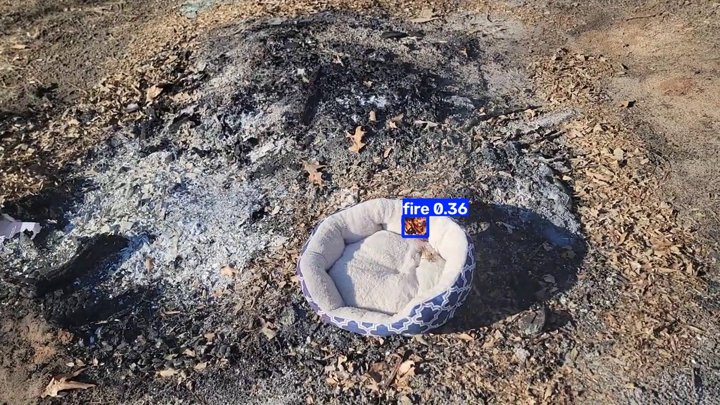
\includegraphics[height=0.22\textheight]{assets/pred_example1.jpg}\hfill
    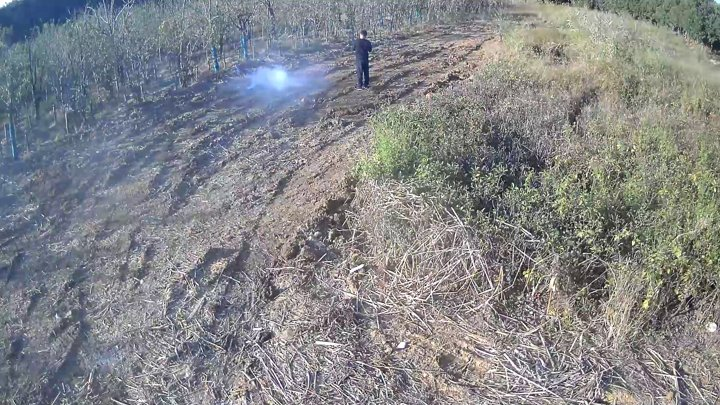
\includegraphics[height=0.22\textheight]{assets/pred_example2.jpg}\hfill
    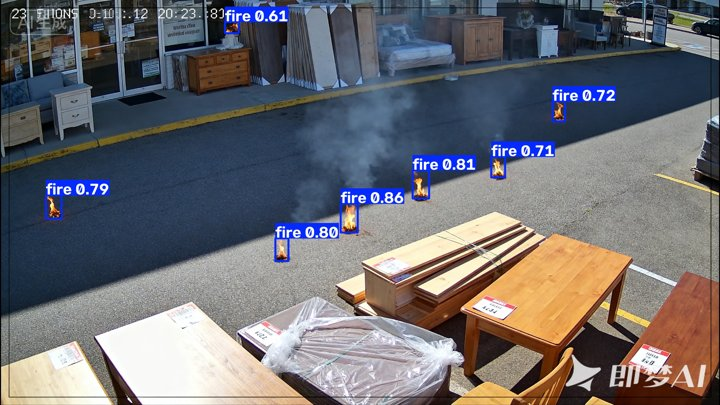
\includegraphics[height=0.22\textheight]{assets/pred_example3.jpg}
  \end{center}
\end{frame}

% ================= 第10页 总结与后续工作 =================
\begin{frame}{总结与后续工作}
  \begin{block}{总结}
    \small
    \begin{itemize}
      \item 已构建完整的监控图像火情识别系统
      \item 已打通数据处理、模型训练、融合推理与结果校验链路
      \item 系统兼顾识别能力与批处理可靠性
    \end{itemize}
  \end{block}
  \begin{block}{后续方向}
    \small
    \begin{itemize}
      \item 面向更多真实监控场景扩展验证
      \item 探索实时视频流处理
      \item 探索轻量化部署方案
    \end{itemize}
  \end{block}
\end{frame}

% ================= 结束页 =================
\begin{frame}[plain]
  \begin{center}
    \vspace{2.5em}
    {\Huge 谢谢！}\\[0.6em]
  \end{center}
\end{frame}

\end{document}
